% \documentclass[12pt]{article}
\documentclass[preprint]{sig-alternate}
% \documentclass[conference]{IEEEtran}

\usepackage{fixacm} % ACM format change
\usepackage[letterpaper,top=1in,bottom=1in,left=1in,right=1in]{geometry}
\usepackage[square,comma,numbers,sort&compress]{natbib}
\usepackage[breaklinks,colorlinks]{hyperref}
\usepackage[usenames,dvipsnames]{color}
\hypersetup{citecolor=blue,linkcolor=blue}
\usepackage{amsmath,amsopn,amssymb}
\usepackage{endnotes,microtype,xspace,graphicx,fancyvrb,multirow}
\usepackage{pgfplots,epsfig,caption,subcaption}
\let\labelindent\relax % stupid IEEE...
\usepackage{enumitem}
\usepackage{grffile}
\usepackage{comment}
% \usepackage{refcheck} % comment this out for final draft
\usepackage{verbatim}
% \usepackage{bigints}
\usepackage{textcomp}
\usepackage{url}
\usepackage[T1]{fontenc}
\usepackage{gensymb}
% \usepackage{authblk} % comment this out for IEEE
\usepackage{breakurl}

% \newcommand{\subparagraph}{}

%%% figs path
\graphicspath{ {figs/} }
\DeclareGraphicsExtensions{.pdf,.png,.jpg}
\setlist[enumerate]{itemsep=0mm}

\def\UrlBreaks{\do\/\do-}
\hypersetup{
     colorlinks   = true,
     citecolor    = blue,
     linkcolor    = magenta
}

\newcommand{\degrees}{$\!\!$\char23$\!$}
\newcommand{\nw}{\newline}
\renewcommand{\refname}{\centerline{REFERENCES CITED}}
% \titlespacing*{\subsection}{0pt}{1.1\baselineskip}{\parskip}
% this handles hanging indents for publications
\def\rrr#1\\{\par
\medskip\hbox{\vbox{\parindent=2em\hsize=6.12in
\hangindent=4em\hangafter=1#1}}}
\def\baselinestretch{1}

\newenvironment{ppl}{\fontfamily{cmr}\selectfont}{\par}
% \newcommand{\superscript}[1]{\ensuremath{^{\textrm{#1}}}}
% \def\sharedaffiliation{\end{tabular}\newline\begin{tabular}{c}}

\renewcommand{\ttdefault}{pxtt}
\newcommand{\URL}{\url}
\newcommand{\cc}[1]{\mbox{\smaller[0.5]\texttt{#1}}}

%\clubpenalty=10000
%\widowpenalty=10000

%\linespread{1.2}

\fvset{fontsize=\scriptsize,xleftmargin=8pt,numbers=left,numbersep=5pt}


\makeatletter
\def\PY@reset{\let\PY@it=\relax \let\PY@bf=\relax%
    \let\PY@ul=\relax \let\PY@tc=\relax%
    \let\PY@bc=\relax \let\PY@ff=\relax}
\def\PY@tok#1{\csname PY@tok@#1\endcsname}
\def\PY@toks#1+{\ifx\relax#1\empty\else%
    \PY@tok{#1}\expandafter\PY@toks\fi}
\def\PY@do#1{\PY@bc{\PY@tc{\PY@ul{%
    \PY@it{\PY@bf{\PY@ff{#1}}}}}}}
\def\PY#1#2{\PY@reset\PY@toks#1+\relax+\PY@do{#2}}

\expandafter\def\csname PY@tok@gd\endcsname{\def\PY@tc##1{\textcolor[rgb]{0.63,0.00,0.00}{##1}}}
\expandafter\def\csname PY@tok@gu\endcsname{\let\PY@bf=\textbf\def\PY@tc##1{\textcolor[rgb]{0.50,0.00,0.50}{##1}}}
\expandafter\def\csname PY@tok@gt\endcsname{\def\PY@tc##1{\textcolor[rgb]{0.00,0.27,0.87}{##1}}}
\expandafter\def\csname PY@tok@gs\endcsname{\let\PY@bf=\textbf}
\expandafter\def\csname PY@tok@gr\endcsname{\def\PY@tc##1{\textcolor[rgb]{1.00,0.00,0.00}{##1}}}
\expandafter\def\csname PY@tok@cm\endcsname{\let\PY@it=\textit\def\PY@tc##1{\textcolor[rgb]{0.25,0.50,0.50}{##1}}}
\expandafter\def\csname PY@tok@vg\endcsname{\def\PY@tc##1{\textcolor[rgb]{0.10,0.09,0.49}{##1}}}
\expandafter\def\csname PY@tok@m\endcsname{\def\PY@tc##1{\textcolor[rgb]{0.40,0.40,0.40}{##1}}}
\expandafter\def\csname PY@tok@mh\endcsname{\def\PY@tc##1{\textcolor[rgb]{0.40,0.40,0.40}{##1}}}
\expandafter\def\csname PY@tok@go\endcsname{\def\PY@tc##1{\textcolor[rgb]{0.53,0.53,0.53}{##1}}}
\expandafter\def\csname PY@tok@ge\endcsname{\let\PY@it=\textit}
\expandafter\def\csname PY@tok@vc\endcsname{\def\PY@tc##1{\textcolor[rgb]{0.10,0.09,0.49}{##1}}}
\expandafter\def\csname PY@tok@il\endcsname{\def\PY@tc##1{\textcolor[rgb]{0.40,0.40,0.40}{##1}}}
\expandafter\def\csname PY@tok@cs\endcsname{\let\PY@it=\textit\def\PY@tc##1{\textcolor[rgb]{0.25,0.50,0.50}{##1}}}
\expandafter\def\csname PY@tok@cp\endcsname{\def\PY@tc##1{\textcolor[rgb]{0.74,0.48,0.00}{##1}}}
\expandafter\def\csname PY@tok@gi\endcsname{\def\PY@tc##1{\textcolor[rgb]{0.00,0.63,0.00}{##1}}}
\expandafter\def\csname PY@tok@gh\endcsname{\let\PY@bf=\textbf\def\PY@tc##1{\textcolor[rgb]{0.00,0.00,0.50}{##1}}}
\expandafter\def\csname PY@tok@ni\endcsname{\let\PY@bf=\textbf\def\PY@tc##1{\textcolor[rgb]{0.60,0.60,0.60}{##1}}}
\expandafter\def\csname PY@tok@nl\endcsname{\def\PY@tc##1{\textcolor[rgb]{0.63,0.63,0.00}{##1}}}
\expandafter\def\csname PY@tok@nn\endcsname{\let\PY@bf=\textbf\def\PY@tc##1{\textcolor[rgb]{0.00,0.00,1.00}{##1}}}
\expandafter\def\csname PY@tok@no\endcsname{\def\PY@tc##1{\textcolor[rgb]{0.53,0.00,0.00}{##1}}}
\expandafter\def\csname PY@tok@na\endcsname{\def\PY@tc##1{\textcolor[rgb]{0.49,0.56,0.16}{##1}}}
\expandafter\def\csname PY@tok@nb\endcsname{\def\PY@tc##1{\textcolor[rgb]{0.00,0.50,0.00}{##1}}}
\expandafter\def\csname PY@tok@nc\endcsname{\let\PY@bf=\textbf\def\PY@tc##1{\textcolor[rgb]{0.00,0.00,1.00}{##1}}}
\expandafter\def\csname PY@tok@nd\endcsname{\def\PY@tc##1{\textcolor[rgb]{0.67,0.13,1.00}{##1}}}
\expandafter\def\csname PY@tok@ne\endcsname{\let\PY@bf=\textbf\def\PY@tc##1{\textcolor[rgb]{0.82,0.25,0.23}{##1}}}
\expandafter\def\csname PY@tok@nf\endcsname{\def\PY@tc##1{\textcolor[rgb]{0.00,0.00,1.00}{##1}}}
\expandafter\def\csname PY@tok@si\endcsname{\let\PY@bf=\textbf\def\PY@tc##1{\textcolor[rgb]{0.73,0.40,0.53}{##1}}}
\expandafter\def\csname PY@tok@s2\endcsname{\def\PY@tc##1{\textcolor[rgb]{0.73,0.13,0.13}{##1}}}
\expandafter\def\csname PY@tok@vi\endcsname{\def\PY@tc##1{\textcolor[rgb]{0.10,0.09,0.49}{##1}}}
\expandafter\def\csname PY@tok@nt\endcsname{\let\PY@bf=\textbf\def\PY@tc##1{\textcolor[rgb]{0.00,0.50,0.00}{##1}}}
\expandafter\def\csname PY@tok@nv\endcsname{\def\PY@tc##1{\textcolor[rgb]{0.10,0.09,0.49}{##1}}}
\expandafter\def\csname PY@tok@s1\endcsname{\def\PY@tc##1{\textcolor[rgb]{0.73,0.13,0.13}{##1}}}
\expandafter\def\csname PY@tok@sh\endcsname{\def\PY@tc##1{\textcolor[rgb]{0.73,0.13,0.13}{##1}}}
\expandafter\def\csname PY@tok@sc\endcsname{\def\PY@tc##1{\textcolor[rgb]{0.73,0.13,0.13}{##1}}}
\expandafter\def\csname PY@tok@sx\endcsname{\def\PY@tc##1{\textcolor[rgb]{0.00,0.50,0.00}{##1}}}
\expandafter\def\csname PY@tok@bp\endcsname{\def\PY@tc##1{\textcolor[rgb]{0.00,0.50,0.00}{##1}}}
\expandafter\def\csname PY@tok@c1\endcsname{\let\PY@it=\textit\def\PY@tc##1{\textcolor[rgb]{0.25,0.50,0.50}{##1}}}
\expandafter\def\csname PY@tok@kc\endcsname{\let\PY@bf=\textbf\def\PY@tc##1{\textcolor[rgb]{0.00,0.50,0.00}{##1}}}
\expandafter\def\csname PY@tok@c\endcsname{\let\PY@it=\textit\def\PY@tc##1{\textcolor[rgb]{0.25,0.50,0.50}{##1}}}
\expandafter\def\csname PY@tok@mf\endcsname{\def\PY@tc##1{\textcolor[rgb]{0.40,0.40,0.40}{##1}}}
\expandafter\def\csname PY@tok@err\endcsname{\def\PY@bc##1{\setlength{\fboxsep}{0pt}\fcolorbox[rgb]{1.00,0.00,0.00}{1,1,1}{\strut ##1}}}
\expandafter\def\csname PY@tok@kd\endcsname{\let\PY@bf=\textbf\def\PY@tc##1{\textcolor[rgb]{0.00,0.50,0.00}{##1}}}
\expandafter\def\csname PY@tok@ss\endcsname{\def\PY@tc##1{\textcolor[rgb]{0.10,0.09,0.49}{##1}}}
\expandafter\def\csname PY@tok@sr\endcsname{\def\PY@tc##1{\textcolor[rgb]{0.73,0.40,0.53}{##1}}}
\expandafter\def\csname PY@tok@mo\endcsname{\def\PY@tc##1{\textcolor[rgb]{0.40,0.40,0.40}{##1}}}
\expandafter\def\csname PY@tok@kn\endcsname{\let\PY@bf=\textbf\def\PY@tc##1{\textcolor[rgb]{0.00,0.50,0.00}{##1}}}
\expandafter\def\csname PY@tok@mi\endcsname{\def\PY@tc##1{\textcolor[rgb]{0.40,0.40,0.40}{##1}}}
\expandafter\def\csname PY@tok@gp\endcsname{\let\PY@bf=\textbf\def\PY@tc##1{\textcolor[rgb]{0.00,0.00,0.50}{##1}}}
\expandafter\def\csname PY@tok@o\endcsname{\def\PY@tc##1{\textcolor[rgb]{0.40,0.40,0.40}{##1}}}
\expandafter\def\csname PY@tok@kr\endcsname{\let\PY@bf=\textbf\def\PY@tc##1{\textcolor[rgb]{0.00,0.50,0.00}{##1}}}
\expandafter\def\csname PY@tok@s\endcsname{\def\PY@tc##1{\textcolor[rgb]{0.73,0.13,0.13}{##1}}}
\expandafter\def\csname PY@tok@kp\endcsname{\def\PY@tc##1{\textcolor[rgb]{0.00,0.50,0.00}{##1}}}
\expandafter\def\csname PY@tok@w\endcsname{\def\PY@tc##1{\textcolor[rgb]{0.73,0.73,0.73}{##1}}}
\expandafter\def\csname PY@tok@kt\endcsname{\def\PY@tc##1{\textcolor[rgb]{0.69,0.00,0.25}{##1}}}
\expandafter\def\csname PY@tok@ow\endcsname{\let\PY@bf=\textbf\def\PY@tc##1{\textcolor[rgb]{0.67,0.13,1.00}{##1}}}
\expandafter\def\csname PY@tok@sb\endcsname{\def\PY@tc##1{\textcolor[rgb]{0.73,0.13,0.13}{##1}}}
\expandafter\def\csname PY@tok@k\endcsname{\let\PY@bf=\textbf\def\PY@tc##1{\textcolor[rgb]{0.00,0.50,0.00}{##1}}}
\expandafter\def\csname PY@tok@se\endcsname{\let\PY@bf=\textbf\def\PY@tc##1{\textcolor[rgb]{0.73,0.40,0.13}{##1}}}
\expandafter\def\csname PY@tok@sd\endcsname{\let\PY@it=\textit\def\PY@tc##1{\textcolor[rgb]{0.73,0.13,0.13}{##1}}}

\def\PYZbs{\char`\\}
\def\PYZus{\char`\_}
\def\PYZob{\char`\{}
\def\PYZcb{\char`\}}
\def\PYZca{\char`\^}
\def\PYZam{\char`\&}
\def\PYZlt{\char`\<}
\def\PYZgt{\char`\>}
\def\PYZsh{\char`\#}
\def\PYZpc{\char`\%}
\def\PYZdl{\char`\$}
\def\PYZhy{\char`\-}
\def\PYZsq{\char`\'}
\def\PYZdq{\char`\"}
\def\PYZti{\char`\~}
% for compatibility with earlier versions
\def\PYZat{@}
\def\PYZlb{[}
\def\PYZrb{]}
\makeatother


\newcommand{\figrule}{\hrule width \hsize height .33pt}
\newcommand{\coderule}{\vspace{-0.4em}\figrule}

\setlength{\abovedisplayskip}{0pt}
\setlength{\abovedisplayshortskip}{0pt}
\setlength{\belowdisplayskip}{0pt}
\setlength{\belowdisplayshortskip}{0pt}
\setlength{\jot}{0pt}

\def\Snospace~{\S{}}
\renewcommand*\sectionautorefname{\Snospace}
\def\sectionautorefname{\Snospace}
\def\subsectionautorefname{\Snospace}
\def\subsubsectionautorefname{\Snospace}
\def\chapterautorefname{\Snospace}
%\renewcommand{\figurename}{Fig.}
%\def\figureautorefname{\figurename}
% \newcommand{\subfigureautorefname}{\figureautorefname}

%\numberwithin{equation}{section}
\newcommand{\yes}{Y}
\newcommand{\no}{}

% sema
\newcommand{\shl}{\ \cc{<}\cc{<}\ }
\newcommand{\shr}{\ \cc{>}\cc{>}\ }

\if 0
\renewcommand{\topfraction}{0.9}
\renewcommand{\dbltopfraction}{0.9}
\renewcommand{\bottomfraction}{0.8}
\renewcommand{\textfraction}{0.05}
\renewcommand{\floatpagefraction}{0.9}
\renewcommand{\dblfloatpagefraction}{0.9}
\setcounter{topnumber}{10}
\setcounter{bottomnumber}{10}
\setcounter{totalnumber}{10}
\setcounter{dbltopnumber}{10}
\fi

\newif\ifdraft\drafttrue
\newif\ifnotes\notestrue
\ifdraft\else\notesfalse\fi

% ref. http://en.wikibooks.org/wiki/LaTeX/Colors
\newcommand{\TK}[1]{\textcolor{LimeGreen}{TK: #1}}
\newcommand{\XXX}[1]{\textcolor{red}{XXX: #1}}
\newcommand{\TODO}[1]{\textcolor{Melon}{TODO: #1}}

% hide comments
% \renewcommand{\TK}[1]{\ignorespaces}
% \renewcommand{\XXX}[1]{\ignorespaces}
% \renewcommand{\TODO}[1]{\ignorespaces}

%% Ensure ligatures (e.g., ``fine official flag'') can be copy/pasted from PDF.
\input{glyphtounicode}
\pdfgentounicode=1

% \newcolumntype{R}[1]{>{\raggedleft\let\newline\\\arraybackslash\hspace{0pt}}p{#1}}

% include macros
\newcommand{\includepdf}[1]{
  \includegraphics[width=\columnwidth]{#1}
}
\newcommand{\includeplot}[1]{
  \resizebox{\columnwidth}{!}{\input{#1}}
}

% list
\newcommand{\squishlist}{
\begin{itemize}[noitemsep,nolistsep]
  \setlength{\itemsep}{-0pt}
}
\newcommand{\squishend}{
  \end{itemize}
}

\date{}
\toappear{EECS 582: ADVANCED OPERATING SYSTEMS (F’16)}

\begin{document}
%%% TITLE
\title{Pythia: the framework for Speculation on Steroids}

%%% authors for ACM
\numberofauthors{1}
\author{Wesley Comber, HyunJong (Joseph) Lee \\ 
\{wcomber, hyunjong\}@umich.edu}
% \affil[*]{University of Michigan} 
% \renewcommand\Authands{ and }

%%% authors for IEEE
% \author{
%   \IEEEauthorblockN{
%     Name1 \IEEEauthorrefmark{1}, 
%     Name2 \IEEEauthorrefmark{1},
%     Name3 \IEEEauthorrefmark{2}
%   }
%   \IEEEauthorblockA{
%     \IEEEauthorrefmark{1} Affil1\\
%     \{name1, name2\}@affil1.edu
%   }

%   \IEEEauthorblockA{
%     \IEEEauthorrefmark{2} Affil2\\
%     name3@affil2.com
%   }
% }

%%% permission
% \newfont{\mycrnotice}{ptmr8t at 7pt}
% \newfont{\myconfname}{ptmri8t at 7pt}
% \let\crnotice\mycrnotice%
% \let\confname\myconfname%
% \CopyrightYear{2015}
% --- Author Metadata here ---
%\permission{Permission to make digital or hard copies of all or part
%of this work for personal or classroom use is granted without fee
%provided that copies are not made or distributed for profit or
%commercial advantage and that copies bear this notice and the full
%citation on the first page. Copyrights for components of this work
%owned by others than the author(s) must be honored. Abstracting with
%credit is permitted. To copy otherwise, or republish, to post on
%servers or to redistribute to lists, requires prior specific
%permission and/or a fee. Request permissions from
%Permissions@acm.org.} \conferenceinfo{Conf 'XX}{Janurary 1 -1 2000,
%City, State} {\mycrnotice{Copyright is held by the owner/author(s).
%Publication rights licensed to ACM.}}} \copyrightetc{ACM
%\the\acmcopyr} \crdata{978-1-4503-2782-4/14/04\ ...\$15.00.\\
%http://dx.doi.org/10.1145/2578726.2578744}
% --- End of Author Metadata ---



\maketitle
\thispagestyle{empty}
% \onecolumn
% \setlength\parindent{0pt}
\nocite{*}

\begin{abstract}
\label{sec:abs}
Put abstract here
\end{abstract}

\section{Introduction}
\label{sec:intro}
Increasing computing power and hardware specs have transformed users to expect
instantaneous response upon their input. For instance, Shneiderman's work showed
that the pace of human-computer interaction has a significant influence on the
user's subjective experience and more importantly, their workflow (1984).
However, there is an increasing reliance on increasingly larger data retrievals
from geographically remote data stores. 

One way to increase the speed of `user-facing data retrieval' is to use prior
experience to predict what queries users may ask in the future, and then work on
the pre-execution or execution of predicted queries in the background. If the
speculation system predicted correctly, then before the user actually asks for
the predicted query, the systems completes the output and/or pre-execution
operations ahead of time and this results in the user experiencing snappier
interaction with the application.

The issue with this naive speculation is significant cost in the case of
mis-prediction. That is, if underlying system frequently mis-predicts which data
or queries that the user is going to ask for, then it ultimately ends up wasting
a lot of work. A higher level approach to the problem allows us to write smarter
pre-executed subqueries with two things in mind. 

First, the speed of the individual subquery, and also the amount of work that
can be repurposed and reused in case the system predicted incorrectly. This
could potentially result in a system that considers individually slower queries,
that are more general or reusable, which speeds up future queries. Thus we want
to investigate what a `bigger-picture' system could do if it weighs both the
speed of each individual query and also the overall speed of accomplishing the
user's ultimate goal, e.g., what is the user ultimately trying to get done using
several queries. 

The idea of ``speculation on steroids'' is to observe a user's session, the
user's context of thinking, and the semantics of their specific queries (e.g.,
how many many people close my website before fully checking out and purchasing
shoes). And then, based on this illustration of the user, to try and predict the
user's high-level activities, i.e., user ultimately wants to know, what the
customers think of their online-store, etc.

Speculating across the many layers of the system to execute queries that are
predicted to be relevant in the background. For example, predicting that the
user will want the results of a query that reports on how many users close the
website before finishing adding shoes to their shopping cart from the item
page. 

Another interesting feature of taking a higher level approach to a speculation
system, is that we can pre-execute and/or execute queries in a way that can be
shared across current and predicted queries to help save computation resources
and to minimize the amount of work wasted in the case of a mis-prediction.



\section{Motivation}
\label{sec:motiv}

User\-oriented interactive  programs often take following sequence of execution:
\begin{enumerate}
\item Get query (input) from a user
\item Compute the result, while a user anxiously waits for the result (``wait''
time)
\item Pause the program, for a user to ``think''
\item Get next query from a user
\end{enumerate}

Previous works have exploited the ``think'' phase to speculatively compute future
steps, whereas what we propose is by extracting the query at a  higher-level
(i.e., finding the ultimate goal that users wish to accomplish with different
data), then we can speculate in a more intelligent manner. 

We achieve this way of speculation by constructing a model that probabilistically
examines the next several steps within the program and user-interaction graph
and then speculatively computes the most likely steps, based on this ``higher
goal'' prediction. In this way, we remove the ``wait'' time by serving precomputed
results. 

The ultimate notion of speculation on steroids is to draw a general observation
on arbitrary users' actions (choices) in a certain setting (e.g., undergraduate
admissions versus graduate admissions). Speculation on a few selective steps
ahead removes the overhead in precomputing all the possible choices as patterns
over a dataset, and this speculative execution is similar to those over another
distinct dataset. 

Even if the model mis predicts choices, the worst case bound is to compute based
on users' choice {\it just in time}, and that is essentially how interactive
data analysis programs do so presently. So our proposed system would use excess
resources to try and speed up future queries, and in the worst case it will
perform equal to the traditional form of execution that starts after the user
asks for it. 

A short example of `speculation on steroids' is to take a simple
user-interaction with a data-visualization program, that displays rates of
seasonal flu-infection rates across the United States. This data comes from a
remote store that is very far from the user's geographical location and thus
there is a significant 15 to 30 second delay in requesting data and receiving
data. In this example, users scroll their view of the map to the state of
Michigan. From this clue, our speculation system would start preloading the more
detailed epidemiology data for the major cities of Detroit, Ann Arbor, and
Ypsilanti. Thus when the user finally zooms in and selects the city of Detroit,
the city's data is displayed much more quickly than the about half minute delay
to pull the data from the remote server.

Carrying the example further, let us assume that Ann Arbor has a large
population of people with the `B+' blood type, and that there is no blood type
data for the city of Detroit. Many scientists are interested in investigating
whether there is a connection between blood type and susceptibility to the
virus. Let us also assume that we only have excess resources to pre-load the
data for a single city. Based on the user's trace and historical traces through
the program, we are inferring that the user is probably interested in (in
preferential order): Detroit, Ann Arbor, and the relationship between blood-type
and the flu. 

In a traditional speculation system, the `dumb' system would simply predict that
the user will most likely be interested in the biggest city in Michigan,
Detroit, because it is first on our predicted `preference list' and the system
would preload that city's data. However, our proposed higher-level system also
infers the amount of `pre-work' that can be re-used in addition to the
likely-hood of the pre-work being used. 

In this system, a possibility for speculative execution, in this case preloading
the detailed city data for Ann Arbor would be chosen for pre-work because even
though the single probable chance that the user is interested in the city of Ann
Arbor's data, is less than the chance that they are interested in Detroit, we
can re-use the `mis-predicted' Ann Arbor data on the off-chance that the user is
actually interested in the blood types of Michigan's cities. 

Thus, despite the fact that `pre-work A' (Detroit data) is slightly more likely
to be requested, we actually do `pre-work B' (Ann Arbor data) because the Ann
Arbor data consists of data that is more-reusable. By taking a higher-level view
of speculation we can choose to do pre-work that is more likely to be used, and
also consider the amount of wasted pre-work that can be reused in the case of a
mis-prediction.



\section{Discussion}
\label{sec:discuss}
In this section, we discuss about the general thoughts behind design and
implementation of our framework {\it Pythia}.

Our system abstracts the idea of speculative execution to the more general idea
of {\it pre-work}s. 
Across many domain spaces, speculative execution can entail many different
things such as pre-fetching from hard disk to memory, pre-fetching the results
of a predicted query from a remote web server, and pre-computing the results of
a predicted query on local data. 
This causes unnecessary complication and complexity for the application
developers who are interested in using excess resources to do some work
ahead-of-time. 

Pre-works are a higher-level concept that encompasses not only the aforementioned
speculative execution use-cases but also considers more abstract concepts such
as the `potential reusability' of pre-works and the system's current excess
resources. 
Thus, {\it Pythia} is a framework that trades excess resources for
improved responsiveness and improved user-experience, thereby applying 
speculative execution to many different applications.

% Due to the limited time-constraints of this class, our class project had
% limited scope with regards to the original higher-level idea of `Speculation
% on Steroids'. One limitation of our current work is that the speculation only
% happens with our single implemented application. One of the core-motivations
% behind the project, was to create a generic speculation framework that
% provides significant benefit across many diverse applications. To have more
% evidence of our system providing this `general speculation framework', we
% would like to test our system across multiple applications and then benchmark
% the performance on each application. 

% Another limitation of the project was the difficulty in finding real data sets
% of user’s traces through an application. We spent the first half of the
% semester trying to find public and/or academic datasets from Google, Facebook,
% and Microsoft to no avail. Ultimately, we settled on using the academic Yelp
% data-set as a candidate application for generalized speculation, but because
% we didn’t have exact user-traces through their application, we still
% encountered some issues with this approach. 

% We ended up having to utilize an analogous heuristic composed of the
% restaurant’s ratings and common reviewers shared between restaurants-- instead
% of exact user’s paths through the program. This let us implement an interactive
% system in time for the class, but also limits the conclusions we can derive from
% the system because it is another level of abstraction from the true generalized
% speculation based on user-traces that our original idea proposed.

\section{Design}
\label{sec:design}

\section{Implementation}
\label{sec:impl}

\section{Evaluations}
\label{sec:eval}

\begin{figure}
  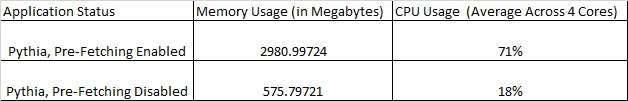
\includegraphics[width=\linewidth]{applicationResourceUsageTable1.jpg}
  \caption{A Table depicting the Main memory and CPU Usage of Our Application with Prefetching enabled and disabled.}
  \label{fig:table1}
\end{figure}

\begin{figure}
  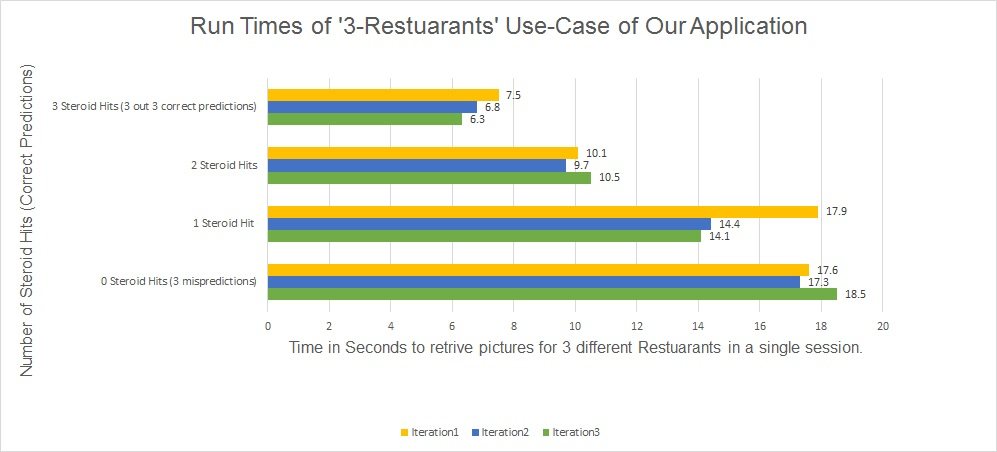
\includegraphics[width=\linewidth]{runTimeChart1.jpg}
  \caption{A Graph depicting runtimes of our Application clustered by Number of Steroid Hits (Correct Predictions).}
  \label{fig:graph1}
\end{figure}


Our evaluation answers two key questions about our system:
\begin{itemize}
\item How much does Pythia speed up the user perceived latency? (In the best case scenario? And in the worst case?)
\item How many excess resources does our implemented system consume? (Is the resource-consumption trade-off worth the speed up?)
\end{itemize}

We used a single Lenovo and IBM Thinkpad x220 for the client machine for running the implemented application. The Thinkpad personal computer has a 'Intel® Core™ i5-2520M (2.5GHz, 3MB L3 cache)', 16GB of DRAM, and a 240 GB solid state hard drive. The machine has a 'ThinkPad 11b/g/n Wireless LAN Mini-PCI Express Adapter II' network adapter. We run the application 12 times on Ubuntu version 14.04.5 LTS with kernel version 3.19. We ran the experiment in two different configurations, one with prefetching enabled and the other with prefetching turned off. The table in Figure 1 shows that disabling the prefetching feature significantly reduces both the memory usage and the CPU usage of our program. In other words, the implemented speculative execution system captures and uses the excess RAM and CPU cycles that would have otherwise been wasted while the user was thinking. Turning off the speculation feature reduces memory usage from almost 3 Gigabytes to a little over one-half of a gigabyte. Likewise for CPU Usage, the Average CPU load across 4 cores is reduced by a factor of almost 4; from 71 percent usage to 18 percent processor usage.

Figure 2 illustrates the relationship between number of accurate predictions and user-perceived response latency for our application. In the 3 cases where all Steroids hit, (in other words, that our application correctly predicted and prefetched the images for all 3 of the 3 restaurants the user explored) the user's session gets sped up from a 17.6, 17.3, and 18.5 second run-time to 7.5, 6.8, and 6.3 second run-times respectively. This is a significant speed up! Our speculative execution system speeds up the user's session by an order of magnitude, specifically improving the user-experience with our application as an interactive session. In the Worst case, where all of our Steroids miss (In other words, all of predictions were wrong and the prefetched data is not used) we simply fetch at request time, and thus deliver latency similar to the case where speculation is turned off. So at best we save 10 seconds in a traditionally 18-second user session, and at worst we take 18 seconds in a traditionally 18-second user session. 

\section{Future Works}
\label{sec:future}

Future work to be done in the project is to apply the system to multiple applications across a diverse domain space. One of the key limitations of project due to time-constraints and limited sources of data and/or user-traces, was that our implemented system only works in the single Yelp restaurant application. Our proposed generalized system is intended to provide a general framework for speculative 'pre-work' that significantly improves user-perceived latency across many different applications. To confirm that our system does effectively generalize across many applications, we would like to implement Pythia on a series of applications and then benchmark their performance, resource usage, and user-perceived latency for the interative applications. 

Another idea worth exploring is using machine learning or iterative Hidden Markov Machines (HMMS) to generate models of weighted probabilistic user-trace paths through the applications. This would let our system dynamically respond to the common user's paths through the application and change accordingly. We would have to make sure we have a significant amount of training data and test data to deal with overfitting issues with the speculative execution. Finally the other future work to be investigated is the greater practicality and efficiency of re-using mispredicted work. We didn't get to implementing re-use of mispredicted work in our project, but we think it is a promising feature based on prior works. By implementing the recycling of mis-predicted and traditionally unused pre-computation, we could more accurately evaluate the benefits and trade-offs of the approach. If the results are promising, and re-using mispredicted work is viable in most applications, then we would introduce that factor into our weighted decision/utility function that determines which work we speculate upon.
\section{Related Works}
\label{sec:related}
The usage of speculative execution for reducing user-perceived latency has a significant history of research and study.  James Mickens, Elson, Howell, and Lorch's 
'Crom' paper from NSDI 2010 explores the role of pre-fetching and speculative execution within the web application and distributed systems domain [1]. Their 'Crom' system allowed for a more-generalized pre-computation framework for the traditionally non-speculative javascript event handlers. By running a shadow clone of the user's browsing session and speculating on the shadow, if the user selects a speculated-upon browser context, then their system presents the precomputed result to the user's real web browser. Their results were promising, they showed that the background speculation overhead "easily fits within user think time", and that  speculative significant reduced user-perceived latencies (in this case from 3,427 ms to 399 ms).

Patterson's 1997 paper examined the use of speculative prefetching and caching to hide disk IO time [2]. The authors create a system that asks applications to disclose their access patterns and uses this information to batch I/O, exploit I/O parallelism, and to dynamically prefetch data from the disk to main memory. Patterson's specialized system had promising results with an up to 36 percent speed up on application run-time and with an average speed of 13 percent speed-up across all the tested applications. Korner's 1990 paper investigated the usage of intelligent file caching for a remote distributed file service to reduce and hide the significant network latencies inherent in the remote file system [3]. Along the same lines as the Korner work on hiding network latencies, Davison's 2001 paper explored the current benefits of web cache prefetching, the broad issues and side effects that plague the current approach, and proposes suggestions to alleviate these issues and side effects [4].

In Davison's paper "Assertion: Prefecthing with GET Is Not Good" states that traditional file system and memory system caching frameworks don't apply well to the web caching domain because of a few key unique attributes of the domain space. Web objects have a variable and unknown cacheability which complicates the determination of which objects to pre-cache, web servers are vulnerable to over-commitment in the case of too many users pre-fetching a significant amount of web objects, and the usage of GET for object retrieval is inherently flawed because of the numerous side effects for the content owner and the intendded content receipient.

James Pitkow and Peter Pirolli from Xerox PARC authored a work  on the extraction of a prediction model for user web-surfing paths from a large amount of historical user-traces through their system [5]. The researchers demonstratred that Kth order Markov Models and N-grams can both efficiently store and represent user's paths. Their results showed that a model prediction accuracy can be significantly improved by storing longer path dependencies at the cost of increased storage space. Their paper also explores the usage of longest repeating sequences, or LRS, to reduce the complexity and storage space needed for stored paths.

In their 1996 paper, Venkata N. Padmanabhan and Jeffrey C. Mogul, dynamically examines the server-collected statistics amount typical client access and requests to create prefetching behavior hints for the server's respective clients [6]. Their results show that their user trace-driven predictions for prefetching significantly reduces the average access time for both high-bandwidth and low-bandwidth clients. They noted that the improvement in web object access time also incurred the cost of increased network traffic. Thus another piece of evidence for the argument that generalized execution should allow developers to easily exchange excess resources (network, disk, memory) for a benefit towards file request and access-response time.

The work, "Nectar: Automatic Management of Data and Computation in Datacenters", by Pradeep Kumar Gunda, et al. carried on this motivation for a higher-level view of computation and speculative 'pre-work' [7]. In the paper, Pradeep, Ravindratnath, Thekkath, Yu, and Zhuang designed and implemented a system that more intelligently manages data and computation within the data-center computing environment. Their Nectar system uses the unification of the concepts of data and computation by tagging and associating data with its respective computation. This allows for the automated management of data access, computation budget, and the caching service that is shared across the datacenter.  The key insight that Gunda et al. had was to abstract the idea of computation from the various data that can be pre-executed (or pre-fetched or pre-cached). This novel lens to view the relationship between computation and data within the data center, allowed them to more easily and more intelligently examine potential pre-computations and caching opprotunities for common computations that can be computed only once and then be reused by others.

At the University of Michigan, researchers Benjamin Wester, Peter M.Chen, and Jason Flinn evaluated the cost and benefits of extending support for application-specific speculation into the underlying operating system. In the 2011 paper, they divide the concept of speculative execution into two equal parts: a policy that specifies which operations and values to preemptively compute, and the underlying mechanisms that support speculation such as check-pointing, rollback, and the tracking of causalities. This work represents another step forward into the idea of de-coupling speculative execution from the exact details and minutiae of the specific applications. Their system performed well, for example they hid up to 85 percent of the program load time by predicting the program's launch, and increased SSL connection latency in the FireFox web-browser by 15 percent. Their more application-agnostic system that resides in the operating system significantly speed up user-perceived latencies for a "modest performance trade-off" and it executed only 8 percent slower than a hand-written customized speculative execution implementation for each specific application.

Alspaugh's, Chen's, Lin's, Ganapathi's, Hearst's, and Katz's 2014 paper investigated the improvement of the Splunk data analysis tools based on the significantly large amount of user-trace logs (over 200,000) from the data analytics platform Splunk. Alspaugh's et al.'s analysis found that most Splunk users' actions in their system consisted of filtering, reformatting, and summarizing data. They also noticed that less-skilled users were more dependent on data from logs to propel their decision making. One of the clever ways the authors capture Splunk users' paths through the program is through state machine diagrams with links of weighted probabilities for transitions between states. This research explored the specialized UI tune-ups and customized features that can be implemented to help with their population's common use-cases, but doesn't entertain the idea of generalized speculative execution that is application-agnostic.

The 'Time Warp' operating system from University of California: Los Angeles, reduced the user-perceived latency for distributed simulations by speculating and pre-computing probable simulation queries across the remote-nodes. This system was specialized for the distributed system architecture of their simulations, so they made many domain specific assumptions such as distributed processes being unable to utilize heap storage and remote file caching. A common theme across these prior works is to specially tailor and tightly couple the implementation of the speculative execution to the application that is being speculated upon. 

Jayachandran, Tunga, Kamat, and Nandi's DICE system that used speculative execution and distributed aggregation to enable smoother and more responsive interactive data cube exploration. In their 2014 paper, the authors realized that many users care more about interactive response-times than exact data accuracy, and their system implements this trade-off by selectively sampling the data. Like previous works, the system relies on the assumption that there is a 'thinking' or in this case 'perusing' phase after the user receives results and opportunistically uses this extra time and extra resources to execute and preemptively cache the results of the most probable future queries, based on the previous queries. The implemented DICE had very promising results, with every single test-user noticing and preferring the speed-up version of the application. Their application saved about 7 seconds for each 54 second session. Throughout all of these previous works, their systems either customized and specifically tailored the speculation system with the targeted applications, or only generalized in a limited manner to speed-up perceived latency for common use-cases of their application. Our proposed Pythia system seeks to generalize in a more abstract fashion to decouple the implementation of broader parts of speculative execution from the minute details of each speculating program.

\newpage
%REF
\bibliographystyle{abbrv}
% \bibliographystyle{ieee}
% {\footnotesize{
  \bibliography{ref}
% }}
\balancecolumns

\end{document}
